\documentclass[english, 12pt]{article}
\usepackage[utf8]{inputenc}

\usepackage[left=1in, right=1in, top=1.5in, bottom=1in]{geometry}
\usepackage{fancyhdr, amsmath, amsfonts, amssymb, amsthm, MnSymbol, wasysym, bbm, mathrsfs, graphicx, listings, parskip, float, hyperref, booktabs, subcaption}
\pagestyle{fancy}

\def\Z{\mathbb{Z}}
\def\R{\mathbb{R}}
\def\Q{\mathbb{Q}}
\def\N{\mathbb{N}}
\def\C{\mathbb{C}}
\def\P{\mathbb{P}}
\def\E{\mathbb{E}}
\def\SF{\mathscr{F}}
\def\CF{\mathcal{F}}
\def\ind{\mathbbm{1}}
\def\giv{{\,|\,}}
\def\lf{\left\lfloor}
\def\rf{\right\rfloor}
\def\lc{\left\lceil}
\def\rc{\right\rceil}
\def\eqd{ \stackrel{d}{=} }
\def\d{ \stackrel{d}{\rightarrow} }
\def\var{\text{Var}}
\def\cov{\text{Cov}}
\newcommand{\simiid}{\overset{\textrm{i.i.d.}}{\sim}}
\newcommand{\simind}{\overset{\textrm{ind.}}{\sim}}
\newcommand{\indep}{\raisebox{0.05em}{\rotatebox[origin=c]{90}{$\models$}}}

%% independence
\newcommand\independent{\protect\mathpalette{\protect\independenT}{\perp}}
\def\independenT#1#2{\mathrel{\rlap{$#1#2$}\mkern2mu{#1#2}}}

\title{The Effect of Vaccination on Next-Year Hospital Admission among Older Adults with Diabetes \\
\small \url{https://github.com/erickim/PH252D\_final\_project}}
\author{Denys Dukhovnov, James Duncan, Eric Kim, David Proudman}
\date{May 7, 2018}

\begin{document}

\maketitle

\newpage

\section{Introduction and Background}
Vaccination can be generally thought of as a preventative measure against many common infectious diseases. It is especially relevant for the children and the elderly, whose frailty and vulnerability leave them exposed to major health complications that result from common viruses, like influenza. In this analysis we aim to assess the impact of vaccination on subsequent hospitalization, as a metric for severe health conditions, in the population of older adults, whose overall health is undermined by the chronic diabetes.

It has been consistently shown that influenza vaccination reduces the risk of hospitalization or death in the elderly with type 2 diabetes \cite{Looijmans}. A recent large-scale study, conducted over several years on the elderly patients with type 2 diabetes, reports a 19\% reduction of hospital admissions for patients receiving influenza vaccine \cite{Vamos}. Although influenza is the most common type of immunization among the elderly population, hepatitis B, shingles, and pneumococcal vaccines are also widespread and are recommended by the CDC, particularly for patients with diabetes \cite{CDC1}. 2015-2016 seasonal influenza vaccination rates in adults over age 65 were 63.4\%, despite the 3.3 percentage point decrease from the prior flu vaccination season, and were the highest among all age groups \cite{CDC2}. The 2015 rates for other common vaccines, such as HPV, Hepatitis A and B, Herpes, Tdap and pneumococcal vaccine, have grown or remained relatively stable since 2010, with greatest improvements among the younger segments of the population, with virtually no changes among the elderly \cite{Williams}.

As compared to other age groups who have manifested virtually no change, the general hospitalization rates have shown marked decline among the older Americans 65 years of age or older, for whom the number of inpatient hospital stays decreased by 25\% from just over 35,214 to 26,480 per 100,000 residents \cite{Sun}. Related to the risk of hospitalization, another recent study has challenged the commonplace conclusion of mortality reductions in the elderly as a result of influenza vaccination. The authors attribute some of the evidence to the selection bias, whereby subjects who were not immunized in the last 5 years were less likely to die than those who were immunized multiple times in the same 5-year period, thus suggesting of the effect of frailty/comorbidities on vaccination outcomes \cite{Baxter}.

In terms of the tendency for adults with diabetes to be vaccinated, one study in Spain found that men, suffering from respiratory and heart diseases, and the elderly are much more likely to choose to immunize than younger adults, females, and otherwise healthy individuals \cite{Jimenez-Garcia}. The effect on vaccination likelihood has been studied extensively and is generally concluded to  positively associate with the degree of health literacy, which is, in turn heavily dependent on one’s educational attainment and socioeconomic status \cite{Howard}. Another salient association exists between the medical risk and the likelihood of vaccination inasmuch as the rate of hospitalization. It is difficult to characterize this factor succinctly, especially in the older adult population with a wide range of health complications and comorbidities, however a portion of the medical risk germane to this specific group of people could in part be attributed to medication non-adherence and overdose \cite{Ho,Budnitz} that further aggravate existing health conditions. Moreover, the increased awareness and acknowledgement of one’s frailty or physical vulnerability toward an infectious disease, such as influenza, is shown to positively associate with the rate of immunization among the elderly with chronic health conditions, such as diabetes.

Cardiac and stroke, cerebrovascular, pneumonia/influenza, as well as other cause of death related hospitalizations were found to be diminished significantly with seasonal influenza vaccinations in the group of 65 years old or above. During the flu season these hospitalizations comprise close to 2.2\% of the vaccinated subpopulation, compared to 3\% for the unvaccinated study subjects, compared to the 10\%-15\% overall baseline hospitalization rate \cite{Nichol}. 

\section{The Causal Model and Causal Question}
We thus pose the causal question of interest, what would the effect of the receipt of any vaccination in 2015 on the hospital admission in 2016 be, if all adults 65+ with with diabetes had been vaccinated, as compared to the case where none of these adults had been vaccinated?

\begin{figure}[H]
    \centering
    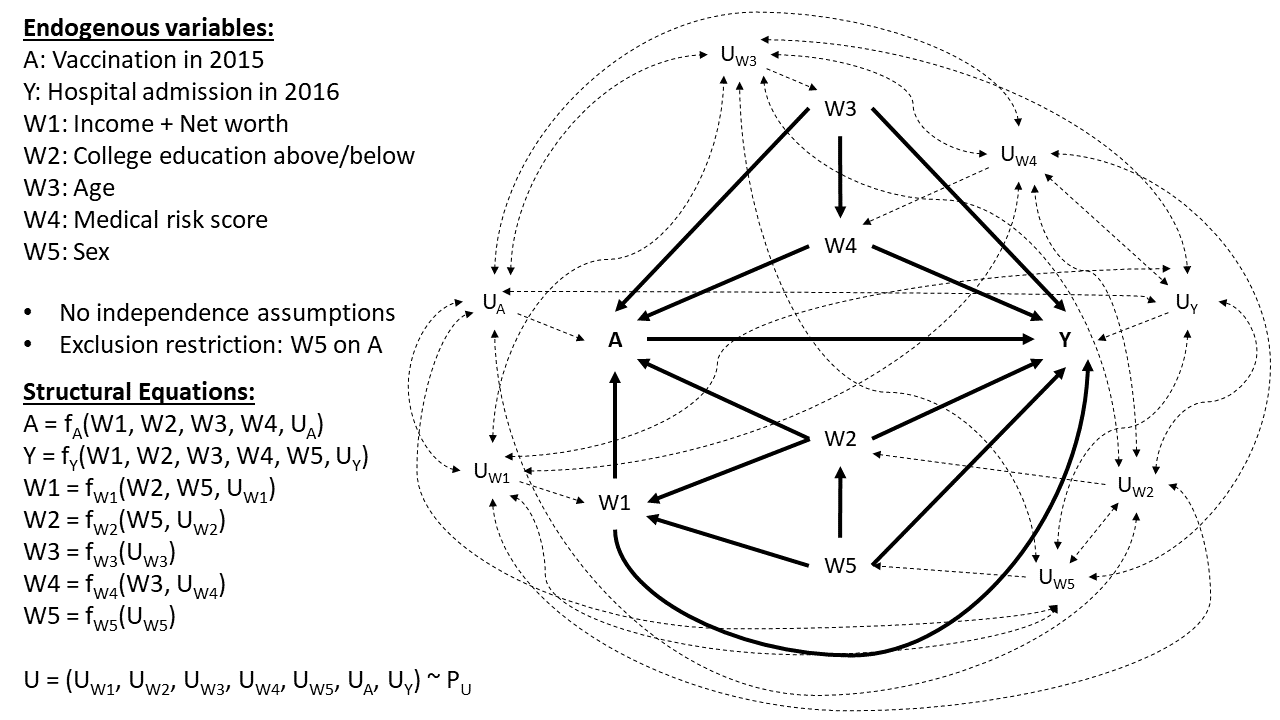
\includegraphics[scale=0.45]{figures/DAG.PNG}
    \caption{Directed acyclic graph showing the proposed structural causal model with structural equations for the effect of vaccination on hospital admission in the following year among older adults with diabetes (2015-2016).}
    \label{fig:DAG_original}
\end{figure}

The base SCM model shown in Figure \ref{fig:DAG_original}. The observed baseline covariates include: income (annual and net worth), binary college education, continuous age in years starting at 65, medical insurance-based continuous medical risk score, and sex. The SCM does not include any independence assumptions, but does contain one exclusion restriction for sex on the vaccination status. The unmeasured background factors $U$ are distributed according to the distribution $P_U$.

The target causal parameter compatible with the model $\mathcal{M}^{\mathcal{F}}$ described in the figure above is the Average Treatment Effect, with the counterfactual outcomes $Y_{1}$ and $Y_{0}$. $$\Psi^F(P_{U,X}) = \E_{U,X}[Y_1-Y_0]$$ The ATE describes the average difference in the counterfactual number of hospital admissions for any reason between the case if adults 65 years old and above with diabetes had they all received at least one immunization in the previous year, as compared to a scenario where none of them were immunized.


\section{Data Description}
In Figure \ref{fig:DAG_original} and Section 2 above, we detail the data obtained from the Texas A\&M University Medical Insurance study that we use in our analysis. For the purpose of this analysis, we further decided to work with the original continuous version of hospital admissions in 2016 as well as a binarized version where the binarized version would give us a measure of the chance of hospitalization. In Table \ref{tab:data_overview}, we see a large summary of the data. With $26779$ overall data points, we show the counts of the binary observed baseline covariates as well as the mean and standard deviations of the continuous variables. We further show the percentage of the subjects in each specific stratum and find that the largest stratum are women with no college education who were not vaccinated while the smallest stratum are men with college education who were vaccinated. While this disparity in the largest and smallest stratum seem shocking, it is important to note that around $78\%$ of the subjects had elected to not receive vaccination and only around $7\%$ of the subjects had a college education. However, even with these asymmetric proportions, because of the large data size, we have a sizable amount of data points for each stratum.

\begin{table}
    \centering
    \resizebox{\columnwidth}{!}{%
    \begin{tabular}{llccccccc}
\toprule
& & \multicolumn{2}{c}{Vaccinated} & \multicolumn{2}{c}{Gender} & \multicolumn{2}{c}{College} & \multicolumn{1}{c}{} \\ \cmidrule(lr){3-4}\cmidrule(lr){5-6}\cmidrule(lr){7-8}
 &  & N & Y & F & M & N & Y & \multicolumn{1}{c}{Overall} \\ 
\midrule
 & count  & $20904$ & $\phantom{0}5875$ & $14055$ & $12724$ & $24843$ & $\phantom{0}1936$ & $26779$ \\
 & \% in stratum  & $78.06\%$ & $21.94\%$ & $52.48\%$ & $47.51\%$ & $92.77\%$ & $\phantom{0}7.23\%$ & $100\%$ \\
Wealth Index & mean  & $11.73$ & $11.94$ & $11.54$ & $12.03$ & $11.75$ & $12.10$ & $\phantom{0}11.78$ \\
 & sd  & $\phantom{0}1.51$ & $\phantom{0}1.53$ & $\phantom{0}1.57$ & $\phantom{0}1.41$ & $\phantom{0}1.51$ & $\phantom{0}1.48$ & $\phantom{00}1.51$ \\
Age & mean  & $74.66$ & $74.68$ & $74.87$ & $74.43$ & $74.75$ & $73.51$ & $\phantom{0}74.66$ \\
 & sd  & $\phantom{0}6.61$ & $\phantom{0}6.32$ & $\phantom{0}6.74$ & $\phantom{0}6.32$ & $\phantom{0}6.57$ & $\phantom{0}6.11$ & $\phantom{00}6.55$ \\
 Medical Risk Score & mean  & $\phantom{0}1.20$ & $\phantom{0}1.11$ & $\phantom{0}1.17$ & $\phantom{0}1.19$ & $\phantom{0}1.18$ & $\phantom{0}1.10$ & $\phantom{00}1.18$ \\
 & sd  & $\phantom{0}0.98$ & $\phantom{0}0.87$ & $\phantom{0}0.94$ & $\phantom{0}0.98$ & $\phantom{0}0.96$ & $\phantom{0}0.96$ & $\phantom{00}0.96$ \\
No. Hospital Visits & mean  & $\phantom{0}0.34$ & $\phantom{0}0.29$ & $\phantom{0}0.32$ & $\phantom{0}0.33$ & $\phantom{0}0.33$ & $\phantom{0}0.28$ & $\phantom{00}0.33$ \\
 & sd  & $\phantom{0}0.94$ & $\phantom{0}0.83$ & $\phantom{0}0.90$ & $\phantom{0}0.93$ & $\phantom{0}0.92$ & $\phantom{0}0.86$ & $\phantom{00}0.92$ \\
\end{tabular}
}
\resizebox{\columnwidth}{!}{%
\begin{tabular}{llcccccccc}
\toprule
& & \multicolumn{8}{c}{Vaccinated} \\ \cmidrule(lr){3-10}
& & \multicolumn{4}{c}{No} & \multicolumn{4}{c}{Yes} \\ \cmidrule(lr){3-6}\cmidrule(lr){7-10}
& & \multicolumn{4}{c}{Gender} & \multicolumn{4}{c}{Gender} \\ \cmidrule(lr){3-6}\cmidrule(lr){7-10}
& & \multicolumn{2}{c}{F} & \multicolumn{2}{c}{M} & \multicolumn{2}{c}{F} & \multicolumn{2}{c}{M} \\ \cmidrule(lr){3-4}\cmidrule(lr){5-6}\cmidrule(lr){7-8}\cmidrule(lr){9-10}
& & \multicolumn{2}{c}{College} & \multicolumn{2}{c}{College} & \multicolumn{2}{c}{College} & \multicolumn{2}{c}{College} \\ \cmidrule(lr){3-4}\cmidrule(lr){5-6}\cmidrule(lr){7-8}\cmidrule(lr){9-10}
 &  & N & Y & N & Y & N & Y & N & \multicolumn{1}{c}{Y} \\ 
\midrule
& count & 10133 & 763 & 9308 & 700 & 2901 & 258 & 2501 & 215 \\
 & \% of total & $37.84\%$ & $2.85\%$ & $34.76\%$ & $2.61\%$ & $10.83\%$ & $0.96\%$ & $9.34\%$ & $0.80\%$ \\
Wealth Index & mean  & $11.47$ & $11.79$ & $11.97$ & $12.27$ & $11.70$ & $12.18$ & $12.15$ & $12.55$ \\
 & sd & $\phantom{0}1.56$ & $\phantom{0}1.52$ & $\phantom{0}1.39$ & $\phantom{0}1.44$ & $\phantom{0}1.58$ & $\phantom{0}1.43$ & $\phantom{0}1.44$ & $\phantom{0}1.34$ \\
Age & mean  & $75.01$ & $73.18$ & $74.45$ & $73.82$ & $74.95$ & $73.42$ & $74.58$ & $73.80$ \\
 & sd  & $\phantom{0}6.83$ & $\phantom{0}6.05$ & $\phantom{0}6.40$ & $\phantom{0}6.28$ & $\phantom{0}6.60$ & $\phantom{0}5.91$ & $\phantom{0}6.04$ & $\phantom{0}6.01$ \\
 Medical Risk Score & mean  & $\phantom{0}1.20$ & $\phantom{0}1.12$ & $\phantom{0}1.20$ & $\phantom{0}1.10$ & $\phantom{0}1.09$ & $\phantom{0}1.00$ & $\phantom{0}1.15$ & $\phantom{0}1.16$ \\
 & sd  & $\phantom{0}0.96$ & $\phantom{0}0.97$ & $\phantom{0}1.00$ & $\phantom{0}1.01$ & $\phantom{0}0.86$ & $\phantom{0}0.81$ & $\phantom{0}0.90$ & $\phantom{0}0.92$ \\
No. Hospital Visits & mean  & $\phantom{0}0.34$ & $\phantom{0}0.30$ & $\phantom{0}0.34$ & $\phantom{0}0.30$ & $\phantom{0}0.28$ & $\phantom{0}0.17$ & $\phantom{0}0.31$ & $\phantom{0}0.25$ \\
 & sd  & $\phantom{0}0.93$ & $\phantom{0}0.95$ & $\phantom{0}0.95$ & $\phantom{0}0.92$ & $\phantom{0}0.82$ & $\phantom{0}0.50$ & $\phantom{0}0.88$ & $\phantom{0}0.66$ \\
\bottomrule 
\end{tabular}
}
    \caption{Data Overview}
    \label{tab:data_overview}
\end{table}


\section{Identifiability}
There is one issue with our currently proposed causal model as we can see in the original DAG of Figure \ref{fig:DAG_original} - we entirely lack identifiability. Due to the expressive nature of the graph and the growing complexity of the nodes and edges, we can easily fail the backdoor-criteria, wherein the treated and untreated individuals are not exchangeable and the assignment of treatment will depend on the potential outcomes. As a result, we will need to make independence assumptions based on background knowledge as follows:
\begin{align*}
U_{A} &\indep U_{W_{3}}, U_{W_{5}} \\
U_{Y} &\indep U_{W_{1}}, U_{W_{2}}, U_{W_{3}}, U_{W_{5}} \\
U_{W_{1}} &\indep U_{W_{3}}, U_{W_{4}}, U_{W_{5}}, U_{Y} \\
U_{W_{2}} &\indep U_{W_{3}}, U_{W_{4}}, U_{W_{5}}, U_{Y} \\
U_{W_{3}} &\indep U_{A}, U_{W_{1}}, U_{W_{2}}, U_{W_{4}}, U_{W_{5}}, U_{Y} \\
U_{W_{4}} &\indep U_{W_{1}}, U_{W_{2}}, U_{W_{3}}, U_{W_{5}} \\
U_{W_{5}} &\indep U_{A}, U_{W_{1}}, U_{W_{2}}, U_{W_{3}}, U_{W_{4}}, U_{Y}
\end{align*}

This is, however, not enough, and we will need the following convenience assumptions:
\begin{align*}
U_{A} &\indep U_{Y}, U_{W_{3}}, U_{W_{4}}, U_{W_{5}} \\
U_{Y} &\indep U_{A}, U_{W_{3}}, U_{W_{5}}
\end{align*}

The DAG with our additional assumptions is shown below in Figure \ref{fig:DAG_updated}.

\begin{figure}[H]
    \centering
    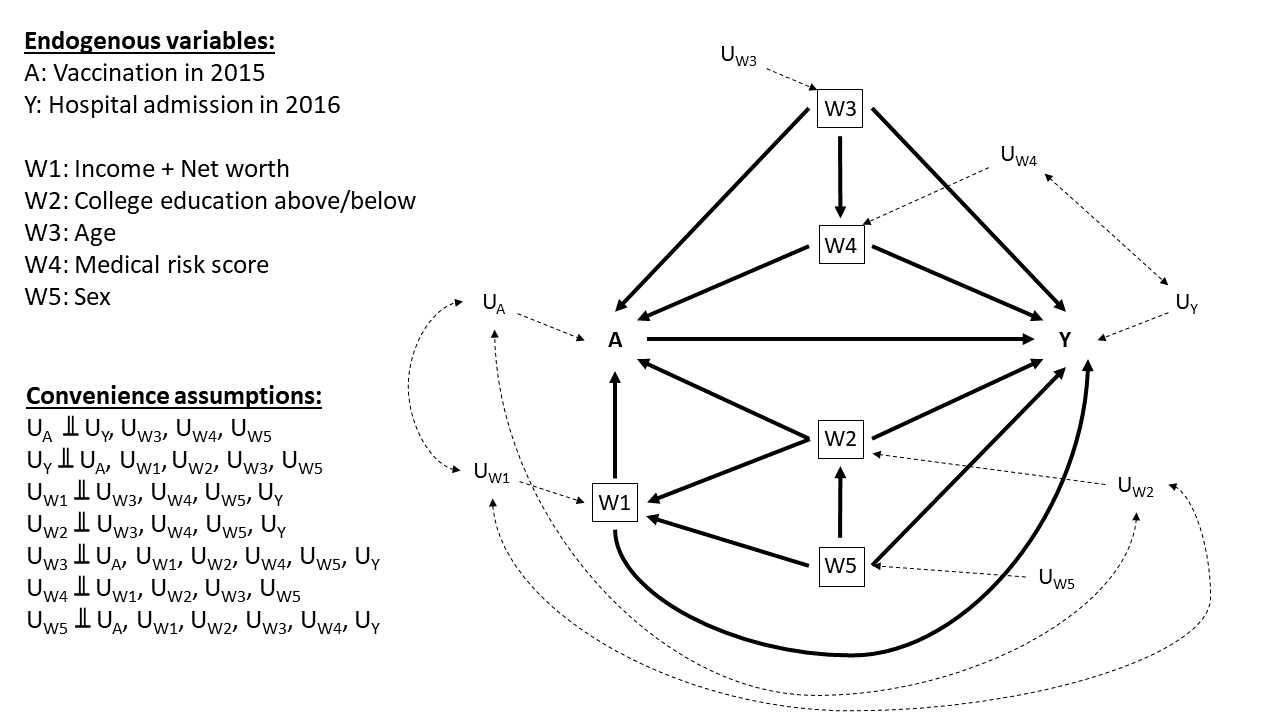
\includegraphics[scale=0.45]{figures/DAG_identifiable.png}
    \caption{Directed acyclic graph showing the structural causal model with independence and convenience assumptions.}
    \label{fig:DAG_updated}
\end{figure}

Our updated SCM $\mathcal{M}^{\mathcal{F}^*}$ restricts the set of observed data distributions $\P_0$ compatible with our model. Every path from $\{W_1,W_2,W_5\}$ to $\{W_3, W_4\}$ is blocked by the colliders $A$ and $Y$, implying that $\{W_1,W_2,W_5\} \independent \{W_3, W_4\}$ in every statistical model compatible with $\mathcal{M}^{\mathcal{F}^*}$. We thus have a semi-parametric statistical model where we have not assumed that there is a finite number of unknown parameters. 

\section{Methodology}

The estimand, or parameter of the observed data distribution, that we have committed to is
    $$\Psi(\P_0) = \E_{W,0} [\E_0(Y|A = 1, W) - \E_0(Y|A = 0, W)]$$
    or equivalently
    $$\Psi(\P_0) = \E_0\left(\frac{\ind\{A = 1\}}{g_0(A=1|W)}Y\right) - \E_0\left(\frac{\ind\{A = 0\}}{g_0(A=0|W)}Y\right).$$
 $\Psi(\P_0)$ is identified with our target causal parameter $\Psi^{\mathcal{F}}(\P_{U,X})$ by the G-computation formula under the convenience assumptions above. The estimators we will use to get an estimate of $\Psi(\P_0)$ are detailed below.

\subsection{Simple Substitution Estimator}

The simple substitution estimator is

$$\hat{\Psi}(\P_n) = \frac{1}{n} \sum_{i=1}^n \bigg[ \hat{\E}\Big(Y_i \giv A_i = 1, W_i = w_i\Big) - \hat{\E}\Big(Y_i \giv A_i = 0, W_i=w_i\Big) \bigg]$$

where $\hat{\E}\Big(Y_i \giv A_i = a, W_i = w_i\Big)$ is the predicted outcome for subject $i$ given (possibly counterfactual) treatment level $a$ and the observed background covariate vector $w_i$. This estimator, based on the G-computation formula, will be consistent for $\Psi(\P_0)$ so long as we consistently estimate $\E_0(Y|A,W)$.

\subsection{Inverse Probability of Treatment Weighted Estimator (IPTW)}

We use two IPTW estimators. The first is the standard Horvitz-Thompson estimator:

$$\hat{\Psi}(\P_n) = \frac{1}{n} \sum_{i=1}^n \frac{\ind\{A_i = 1\}}{g(A_i \giv W_i)} Y_i - \frac{1}{n} \sum_{i=1}^n \frac{\ind\{A_i = 0 \}}{g(A_i \giv W_i)} Y_i.$$

The second is the stabilized Horvitz-Thompson estimator, which can help with near violations of the positivity assumption:

$$\hat{\Psi}(\P_n) = \frac{\sum_{i=1}^n \frac{\ind\{A_i = 1\}}{g(A_i \giv W_i)} Y_i}{\sum_{j=1}^n \frac{\ind\{A_j = 1\}}{g(A_j \giv W_j)}} - \frac{\sum_{i=1}^n \frac{\ind\{A_i = 0 \}}{g(A_i \giv W_i)}Y_i}{\sum_{j=1}^n \frac{\ind\{A_j = 0\}}{g(A_j \giv W_j)}}.$$

In either case, these estimators will be consistent for $\Psi(\P_0)$ so long as we consistently estimate the treatment mechanism $g_0(A|W)$.

\subsection{TMLE}

The TMLE is a substitution estimator which involves estimating both $E_0(Y | A, W)$ and $g_0(A|W)$, resulting in a doubly robust, targeted estimate of $\Psi(\P_0)$. The algorithm is:

\begin{enumerate}
    \item Estimate $\bar{Q}_0(A, W) = E_0(Y | A, W)$ using Super Learner, giving $\bar{Q}_n^0(A, W)$.
    \item Estimate the treatment mechanism $g_0(A|W)$ by Super Learner, giving $g_n(A|W)$.
    \item Define the clever covariate for each subject $i$:
    $$H_n(A_i, W_i) \equiv \left( \frac{\ind\{A_i = 1\}}{g_n(A_i = 1|W_i)} - \frac{\ind\{A_i = 0\}}{g_n(A_i = 0 | W_i)} \right).$$
    \item Run logistic regression with the model
    $$ logit\{E(Y_i|A_i, W_i)\} = logit\{\bar{Q}_n^0(A_i, W_i)\} + \epsilon H_n(A_i, Wi) $$
    to find the estimate $\epsilon_n$ of the clever covariate coefficient that minimizes the squared error loss.
    \item Update the estimate of $\bar{Q}_0(A, W)$:
    $$\bar{Q}^*_n(A, W) = expit\{logit(\bar{Q}_n^0) + \epsilon_n H_n(A,W)\}.$$
    \item Use $\bar{Q}^*_n(A, W)$ to get predicted values under each treatment level for each individual: $\bar{Q}^*_n(1, W_i)$ and $\bar{Q}^*_n(0, W_i)$.
\end{enumerate}

The final estimator for $\Psi(\P_0)$ is
$$\hat{\Psi}(\P_n) = \frac{1}{n}\sum_{i = 1}^n [\bar{Q}^*_n(1, W_i) - \bar{Q}^*_n(0, W_i)]$$
which is consistent if either $E_0(Y | A, W)$ or $g_0(A|W)$ are estimated consistently, and if both are then it is also efficient.

\section{Results}

\subsection{Positivity Assumption}

In order to identify the G-computation formula with $\Psi(P_{U,X})$, we must have

$$ \min_{a \in \mathcal{A}} \P_0(A = a| W = w) > 0,$$

for all $w$ for which $\P_0(W = w) > 0$. In other words, for all values on the support of the joint distribution of the background covariates $W$, there must be a non-zero probability of both levels of treatment (vaccinated/not vaccinated in 2015). As all of our subjects were insured in 2015 and thus had ready access to low-cost or free vaccination, we assume that the theoretical positivity assumption is met.

However, we have to be weary of practical positivity violations or near violations, which can at best make our estimators more variable (high variance weights) and at worst bias our estimators (extrapolation to unobserved regions of $(A, W)$), or even undo identifiability in the case of the G-computation estimator. To evaluate practical positivity we examine the distribution of propensity scores, IPTW weights, and stabilized IPTW weights.

Figure \ref{fig:propensity} shows the distribution of estimated propensity scores $g_n(A = 1 | W)$, the probability of vaccination in 2015 given background covariates, for all 26779 subjects. The minimum and maximum scores are 0.084 and 0.336. Importantly, the scores are neither very small nor very large, and as a result $g_n(A_i = 0|W_i) = 1 - g_n(A_i|W_i)$ will also not be very small. As we will see next, this precludes extreme weights in the IPTW estimators.

\begin{figure}
    \centering
    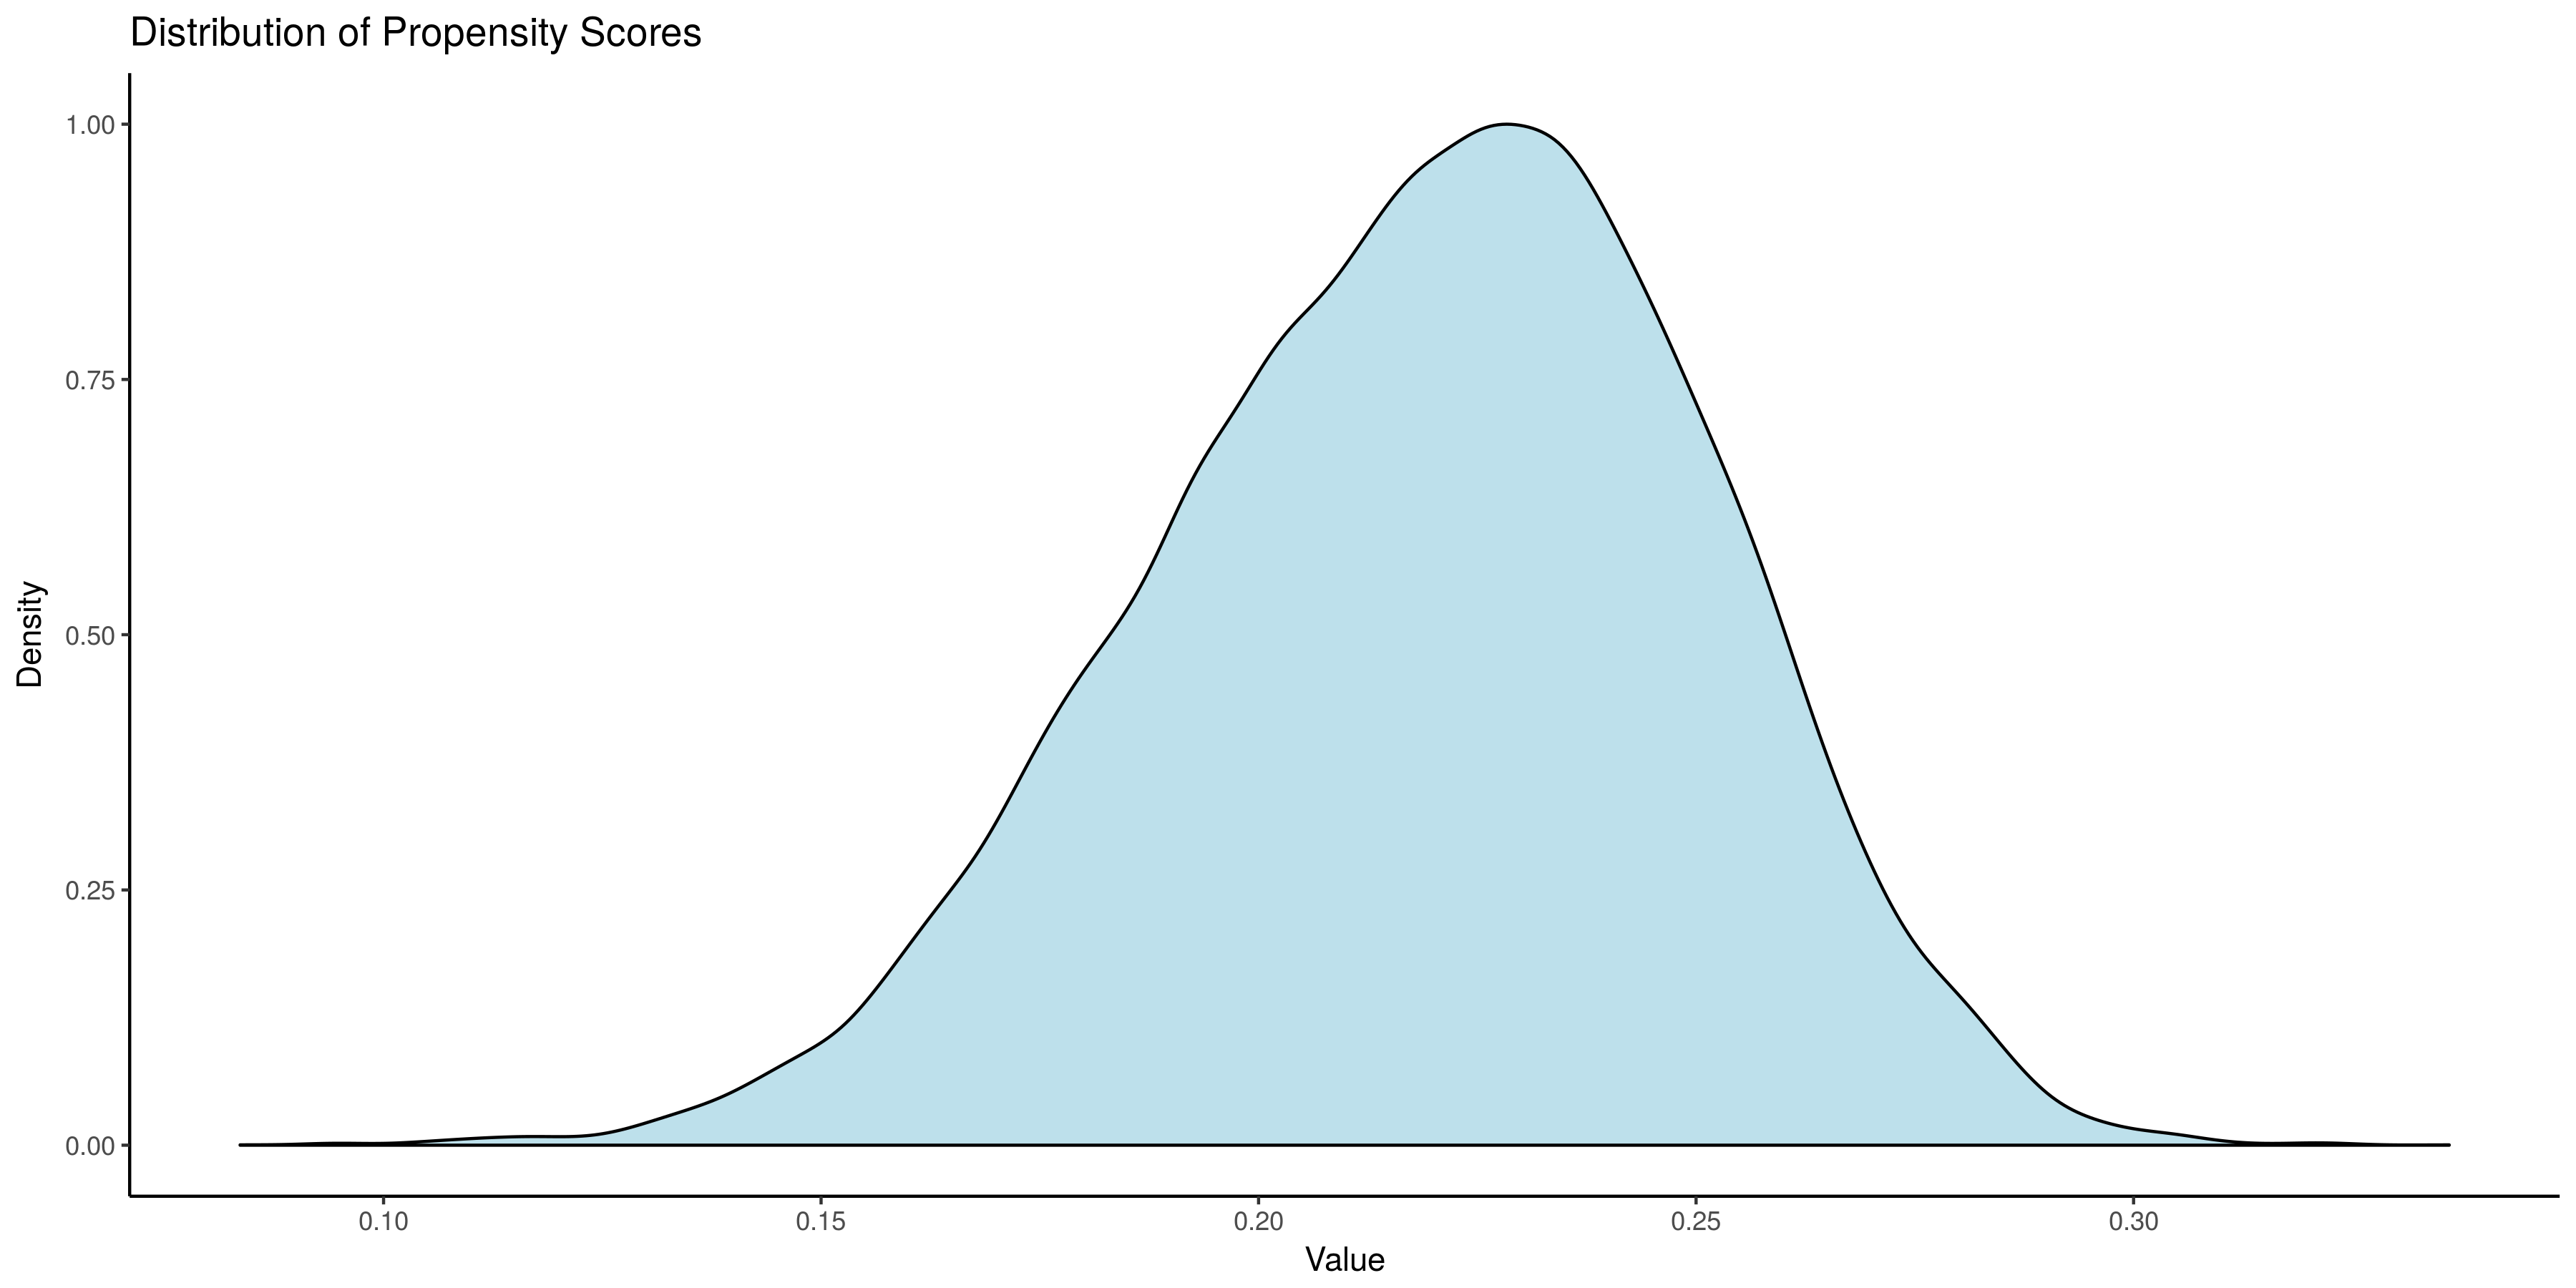
\includegraphics[scale=0.5]{figures/propensity.png}
    \caption{Probability of vaccination in 2015, given background covariates.}
    \label{fig:propensity}
\end{figure}

Figure \ref{fig:IPTW_a} gives the distribution of IPTW weights, defined as
$$\hat{\omega}_i = \frac{1}{g_n(A_i = a_i|W_i)}$$
where $a_i$ is the true vaccination status of subject $i$. The left mode corresponds to the much larger portion of the data that was not vaccinated in 2015. The minimum and maximum of the IPTW weights was 1.09 and 10.7. No weight is unreasonably large and, in combination with the fact that there are no outright violations of positivity, we conclude that the practical positvity assumption is also satisfied.

Figure \ref{fig:IPTW_b} also shows the distribution of the stabilized IPTW weights. The shape of the distribution is remarkably similar to the unstabilized version. This is because the sums in the denominators of the weights for those that were vaccinated and those that weren't were quite close: about 26803 and 26778, respectively. There are far fewer subjects that were vaccinated in 2015 and their weights are higher than the weights of those that were not vaccinated to compensate, balancing the sums.

\begin{figure}
\centering
\begin{subfigure}{\columnwidth}
\centering
    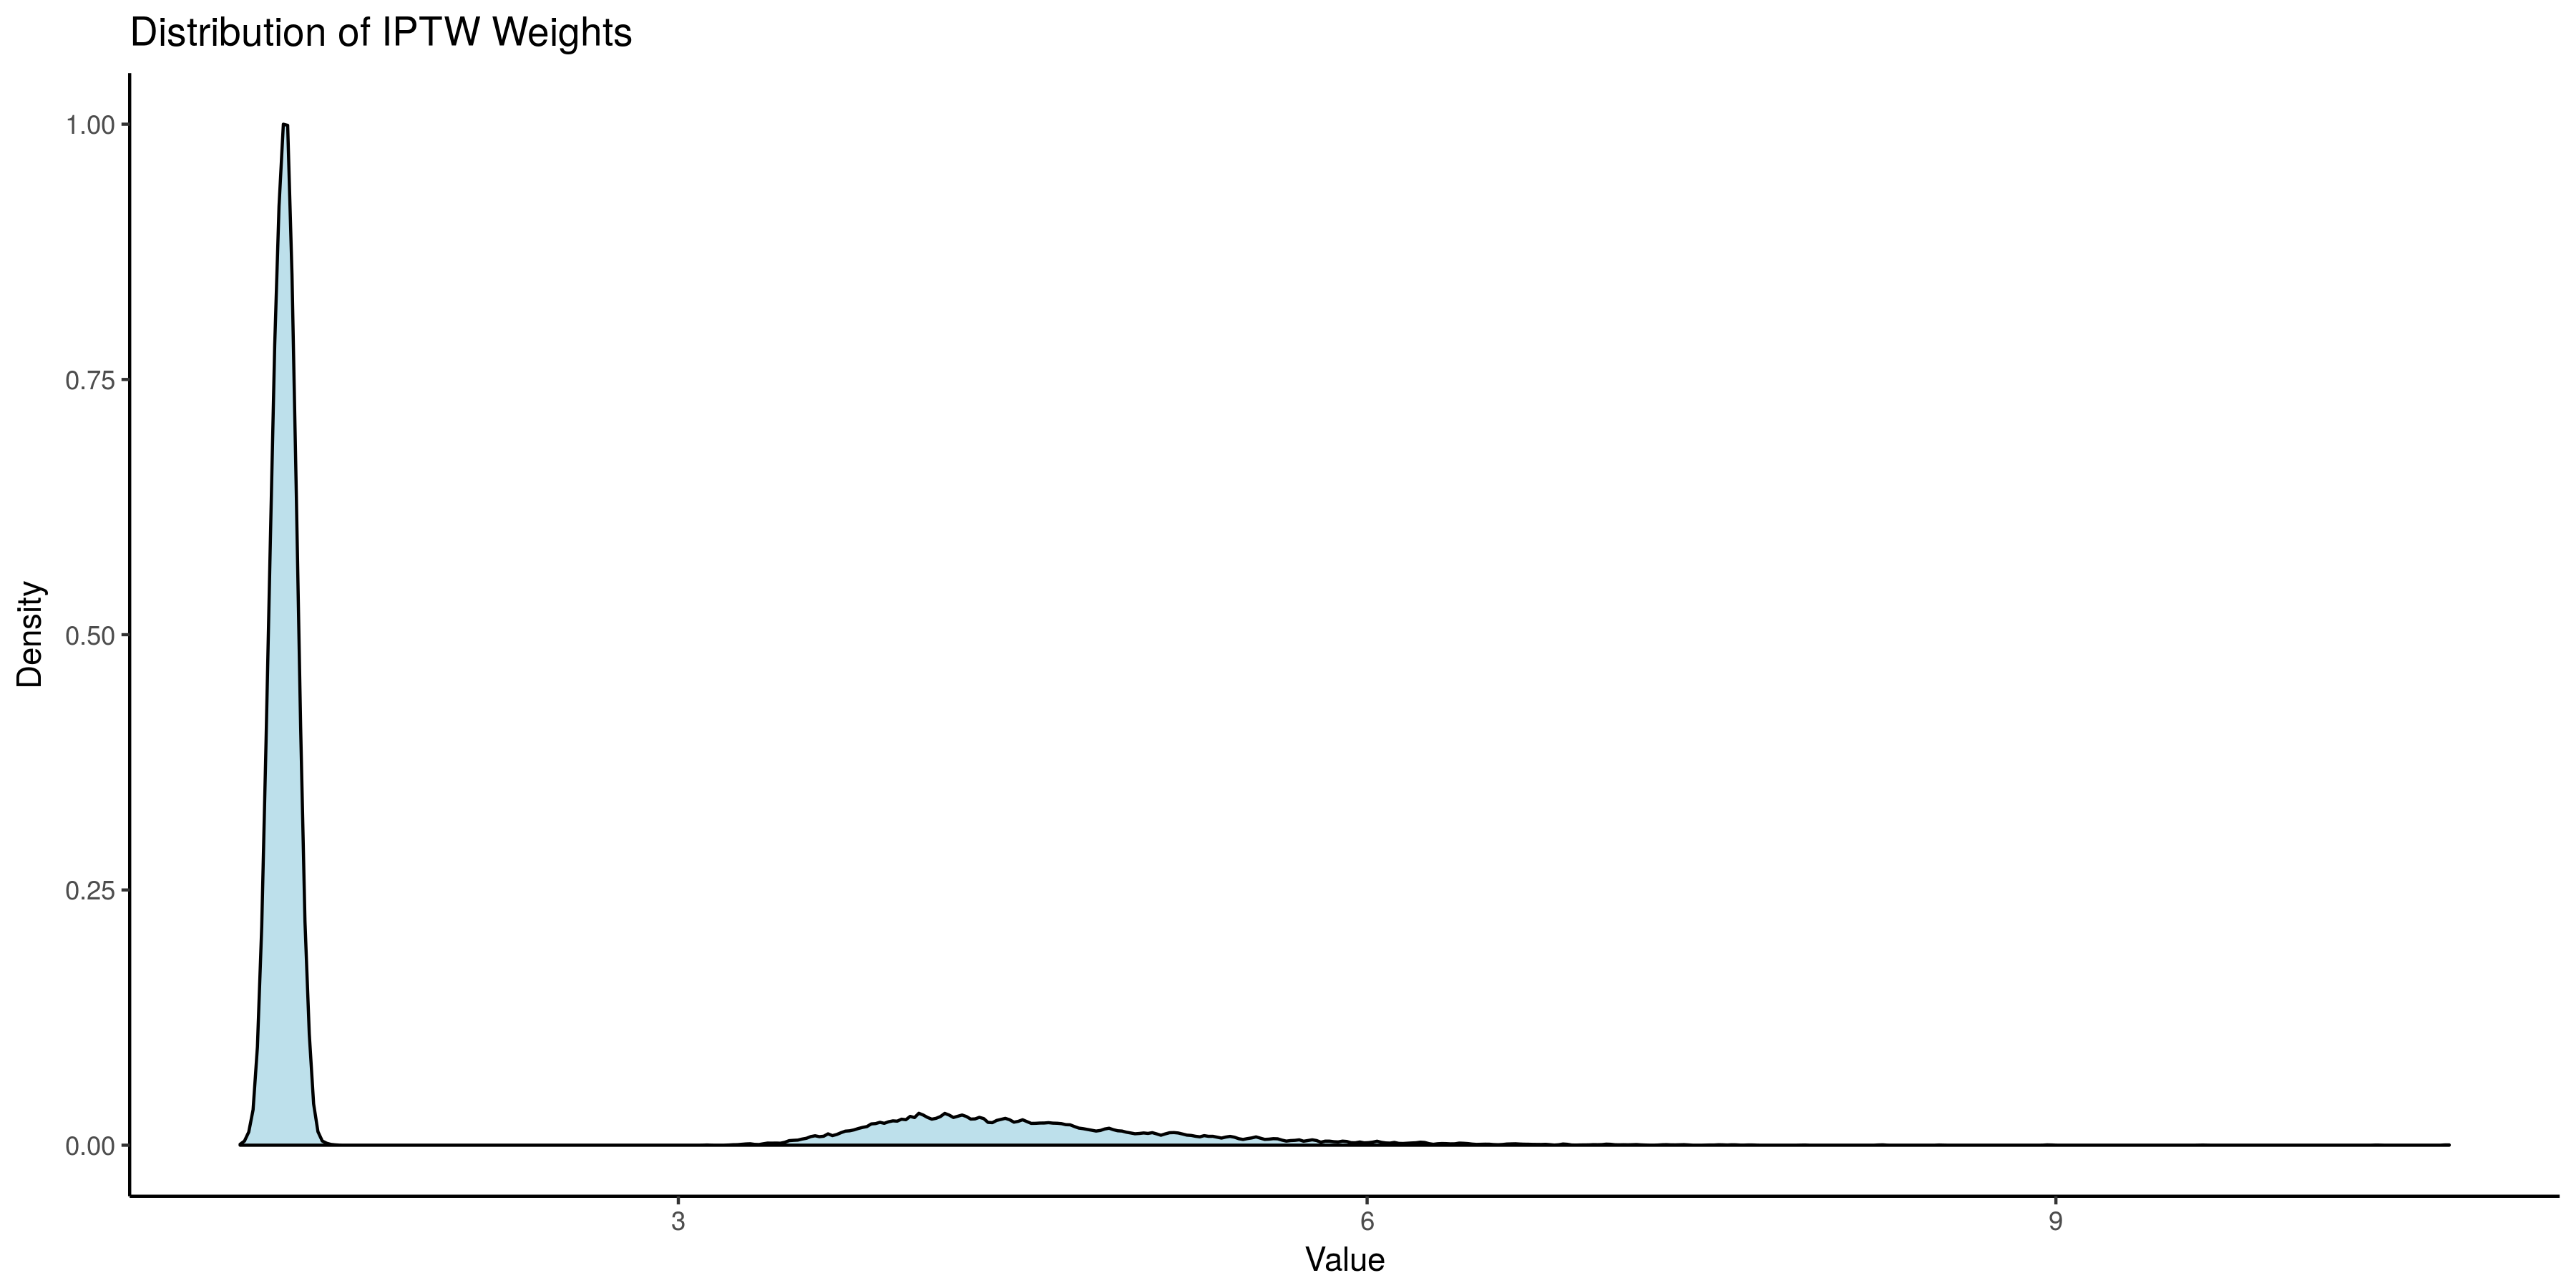
\includegraphics[scale=0.5]{figures/IPTW_weights.png}
    \caption{IPTW Weights}
    \label{fig:IPTW_a}
\end{subfigure}\hspace{0.1in}
\begin{subfigure}{\columnwidth}
\centering
    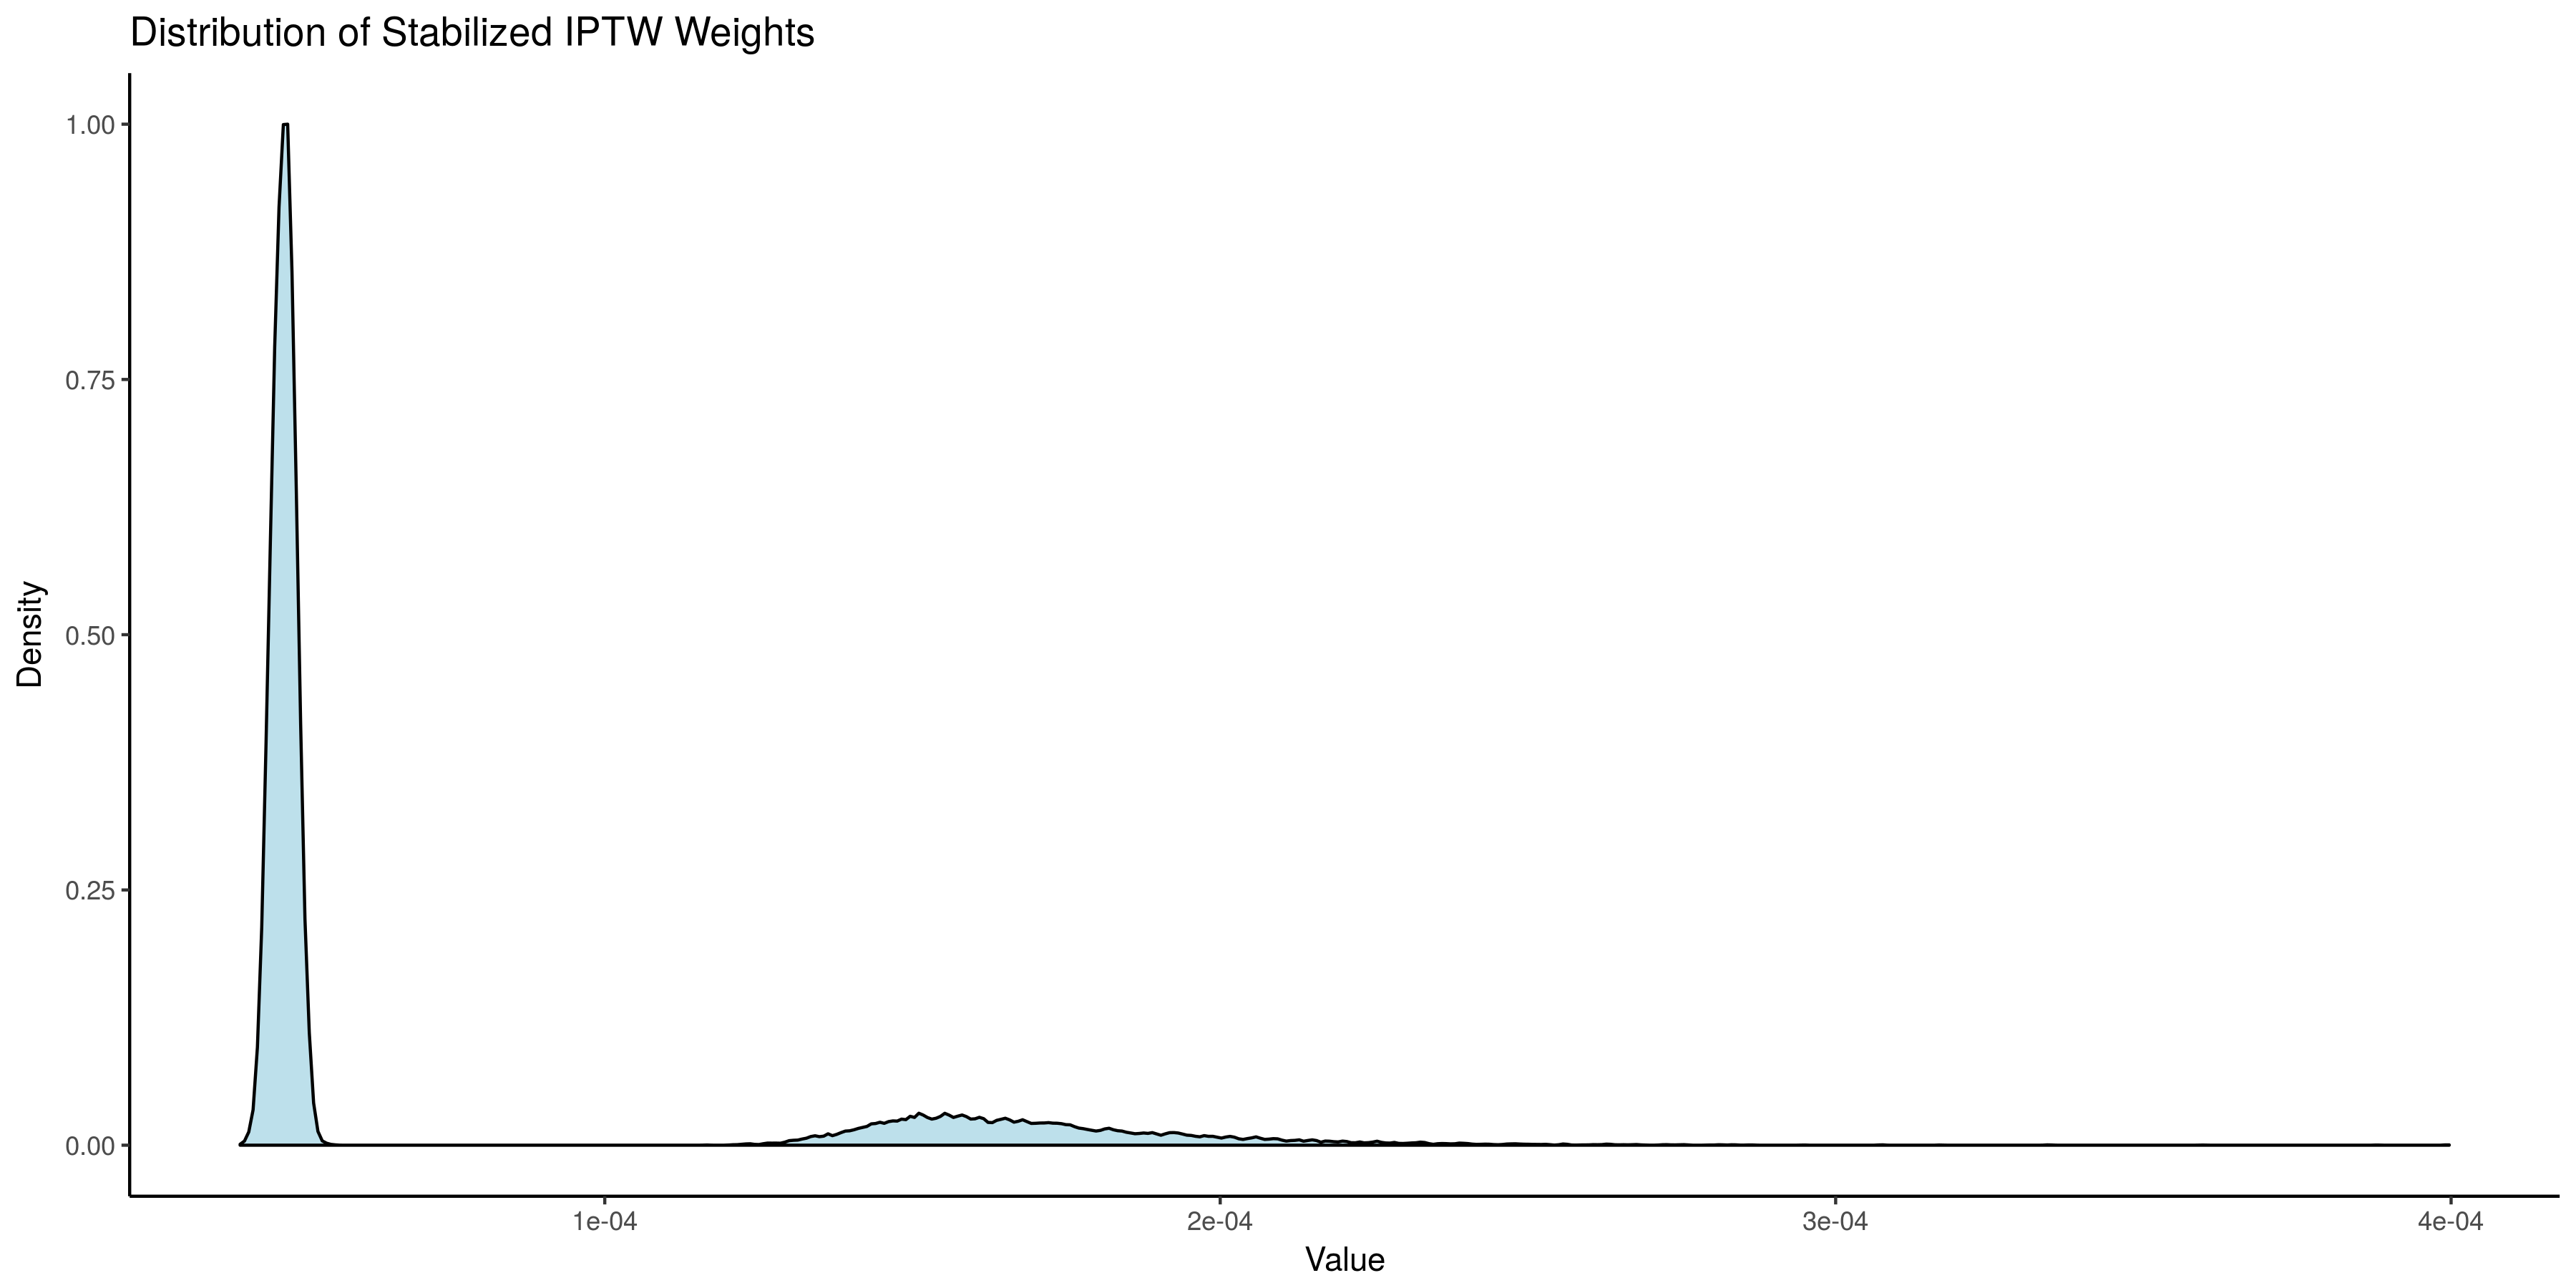
\includegraphics[scale=0.5]{figures/stabilized_IPTW_weights.png}
    \caption{Stabilized IPTW weights.}
    \label{fig:IPTW_b}
\end{subfigure}
\caption{Inverse Probability of Treatment, Weighted}
\label{fig:IPTW}
\end{figure}

\subsection{Estimation}
\begin{table}
\begin{center}
\begin{tabular}{lcccc}
\toprule
 & \multicolumn{4}{c}{Outcome} \\ \cmidrule(lr){2-5}
 & \multicolumn{2}{c}{Binary} & \multicolumn{2}{c}{Continuous} \\ \cmidrule(lr){2-3}\cmidrule(lr){4-5}
Estimand  & $\hat{\Psi}$ & SE & $\hat{\Psi}$ & \multicolumn{1}{c}{SE} \\ 
\midrule
G-Computation  & $-0.0116$ & $\phantom{-}0.00525$ & $-0.0373$ & $\phantom{-}0.0125$ \\
IPTW  & $-0.0127$ & $\phantom{-}0.00534$ & $-0.0394$ & $\phantom{-}0.0130$ \\
Stabilized IPTW  & $-0.0139$ & $\phantom{-}0.00531$ & $-0.0397$ & $\phantom{-}0.0130$ \\
TMLE (SuperLearner)  & $-0.0107$ & $\phantom{-}0.00550$ & $-0.0318$ & $\phantom{-}0.0127$ \\
\bottomrule 
\end{tabular}

\caption{Estimation Results}
\label{tab:estimation}
\end{center}
\end{table}

In Table \ref{tab:estimation} we see the results of our estimation. The standard errors for the G-Computation, IPTW, and Stabilized IPTW for both binary and continuous were computed via the non-parametric bootstrap with 500 bootstrap samples. The standard error reported for TMLE is from the influence curve as computed from the \texttt{ltmle} package via the SuperLearner where our SuperLearner library was the following \texttt{SL.glm, SL.glm.interaction, SL.step, SL.gam, SL.rpartPrune, SL.mean}. We can see that the estimates were all relatively well behaved and similar to each other as it definitely seems like we had Central Limit Theorem working for our large sample size. 

\begin{table}
    \centering
    \begin{tabular}{lcccccccc}
\toprule
 & \multicolumn{4}{c}{Binary} & \multicolumn{4}{c}{Continuous} \\
 \cmidrule(lr){2-5}\cmidrule(lr){6-9}
 & \multicolumn{2}{c}{$g_n$} & \multicolumn{2}{c}{$\bar{Q}_n^0$} & \multicolumn{2}{c}{$g_n$} &  \multicolumn{2}{c}{$\bar{Q}_n^0$} \\
 \cmidrule(lr){2-3}\cmidrule(lr){4-5}\cmidrule(lr){6-7}\cmidrule(lr){8-9}
Name  & cvRisk & coef & cvRisk & coef & cvRisk & coef & cvRisk & \multicolumn{1}{c}{coef} \\ 
\midrule
gam  & $0.170$ & $1$ & $0.135$ & $0.882$ & $0.170$ & $1$ & $0.005$ & $0.389$ \\
glm  & $0.170$ & $0$ & $0.135$ & $0$ & $0.170$ & $0$ & $0.005$ & $0$ \\
glm.interaction  & $0.170$ & $0$ & $0.135$ & $0.049$ & $0.170$ & $0$ & $0.005$ & $0.611$ \\
mean  & $0.171$ & $0$ & $0.144$ & $0$ & $0.171$ & $0$ & $0.006$ & $0$ \\
rpartPrune  & $0.171$ & $0$ & $0.139$ & $0.069$ & $0.171$ & $0$ & $0.011$ & $0$ \\
step  & $0.170$ & $0$ & $0.135$ & $0$ & $0.170$ & $0$ & $0.005$ & $0$ \\
\bottomrule 
\end{tabular}
    \caption{Performance Assessment}
    \label{tab:performance}
\end{table}

Table \ref{tab:performance} shows the cross-validated risk and ensemble learner coefficients for each algorithm in our library when estimating $g_0$ and $\bar{Q}_0$. In the binary outcome case, SuperLearner gives all the weight to \texttt{SL.gam} in estimating $g_0$ and combines \texttt{SL.gam, SL.glm.interaction} and \texttt{SL.rpartPrune} to estimate $\bar{Q}_0$, with \texttt{SL.gam} receiving nearly 90\% of the weight. The continuous case again places all weight on \texttt{SL.gam} when estimating $g_0$, but only chooses \texttt{SL.gam} and \texttt{SL.glm.interaction}, place much less weight on \texttt{SL.gam}, with the majority ($\approx$ 60\%) going to \texttt{SL.glm.interaction}.

The average risk from \texttt{CV.SuperLearner} in the continuous case was 0.789 for Super Learner, followed closely by the discrete winner \texttt{SL.gam} at 0.79. The other algorithms in the library had risk between 0.79 and 0.8, substantially better than the 0.84 risk of \texttt{SL.mean}. Super Learner places non-zero weight on \texttt{SL.gam} and \texttt{SL.rpartPrune}.

In the binary outcome case, the MSE of the ensemble learner was actually $10^{-5}$ higher than \texttt{SL.gam}, but both were around 0.135. The other algorithms also had MSE hovering just above 0.135, other than \texttt{SL.rpartPrune} at 0.141, which was still better than \texttt{SL.mean}'s MSE of 0.144. Super Learner places non-zero weight on \texttt{SL.glm.interaction}, \texttt{SL.gam}, and -- in spite of its poor performance -- a small weight on \texttt{SL.rpartPrune}.

\begin{figure}
\centering
\begin{subfigure}{\columnwidth}
\centering
    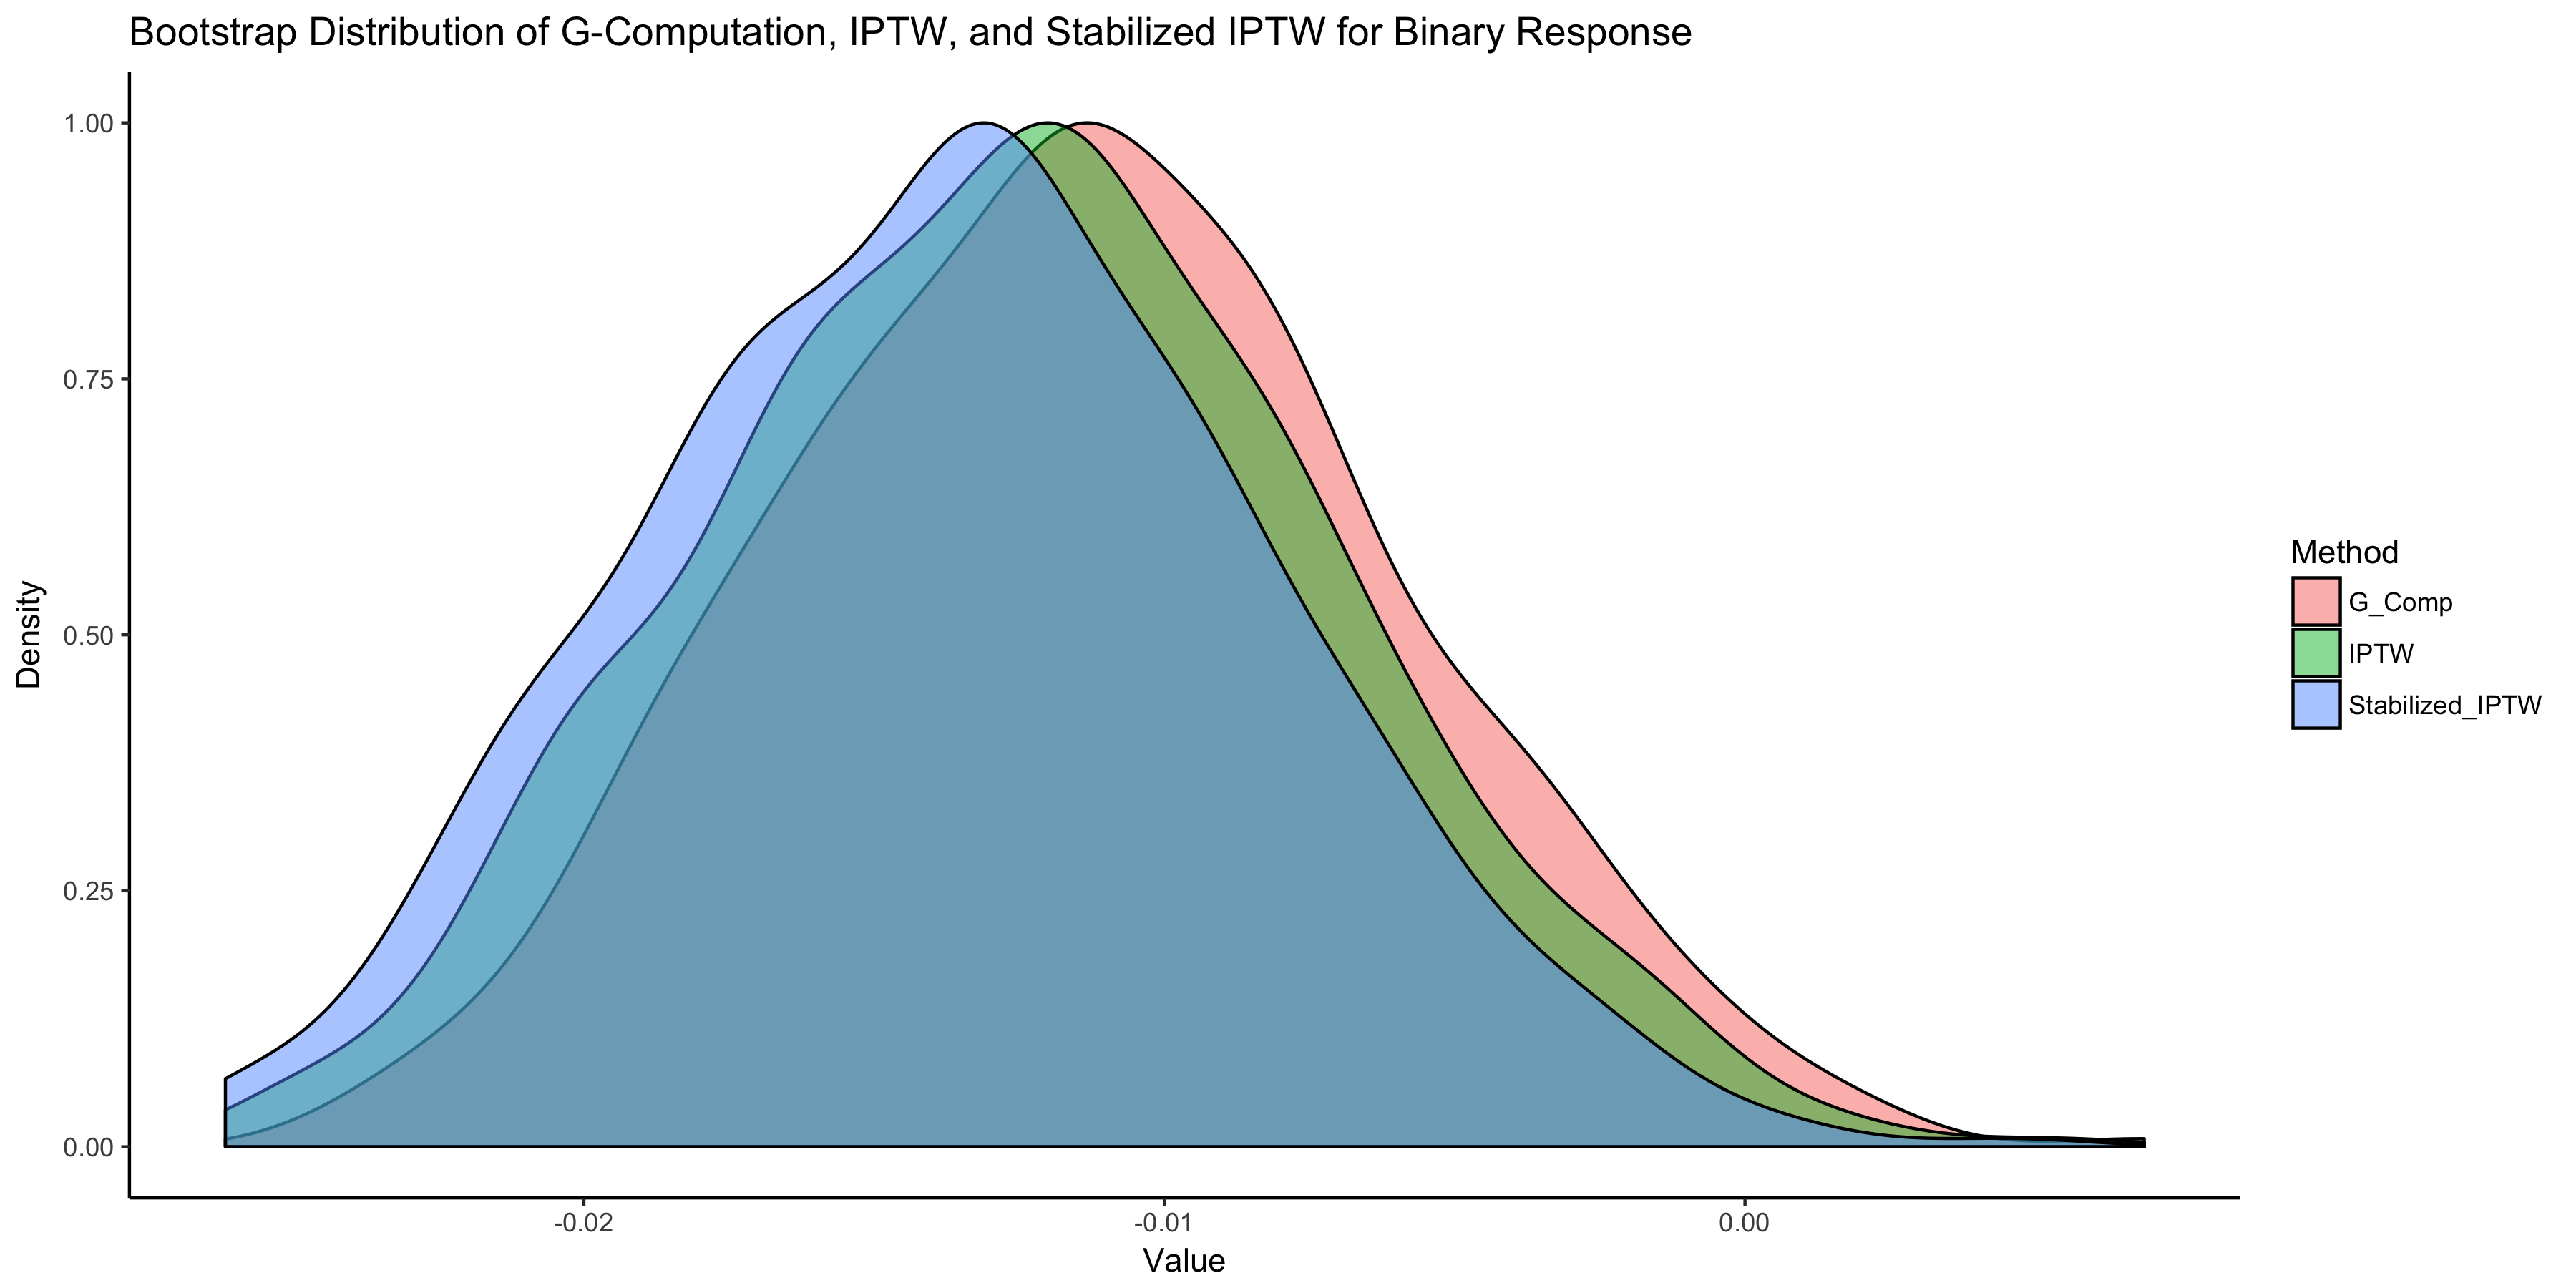
\includegraphics[scale=0.125]{figures/boot_dens_binary.png}    \caption{Binarized Response}
    \label{fig:boot_bin}
\end{subfigure}
\begin{subfigure}{\columnwidth}
\centering
    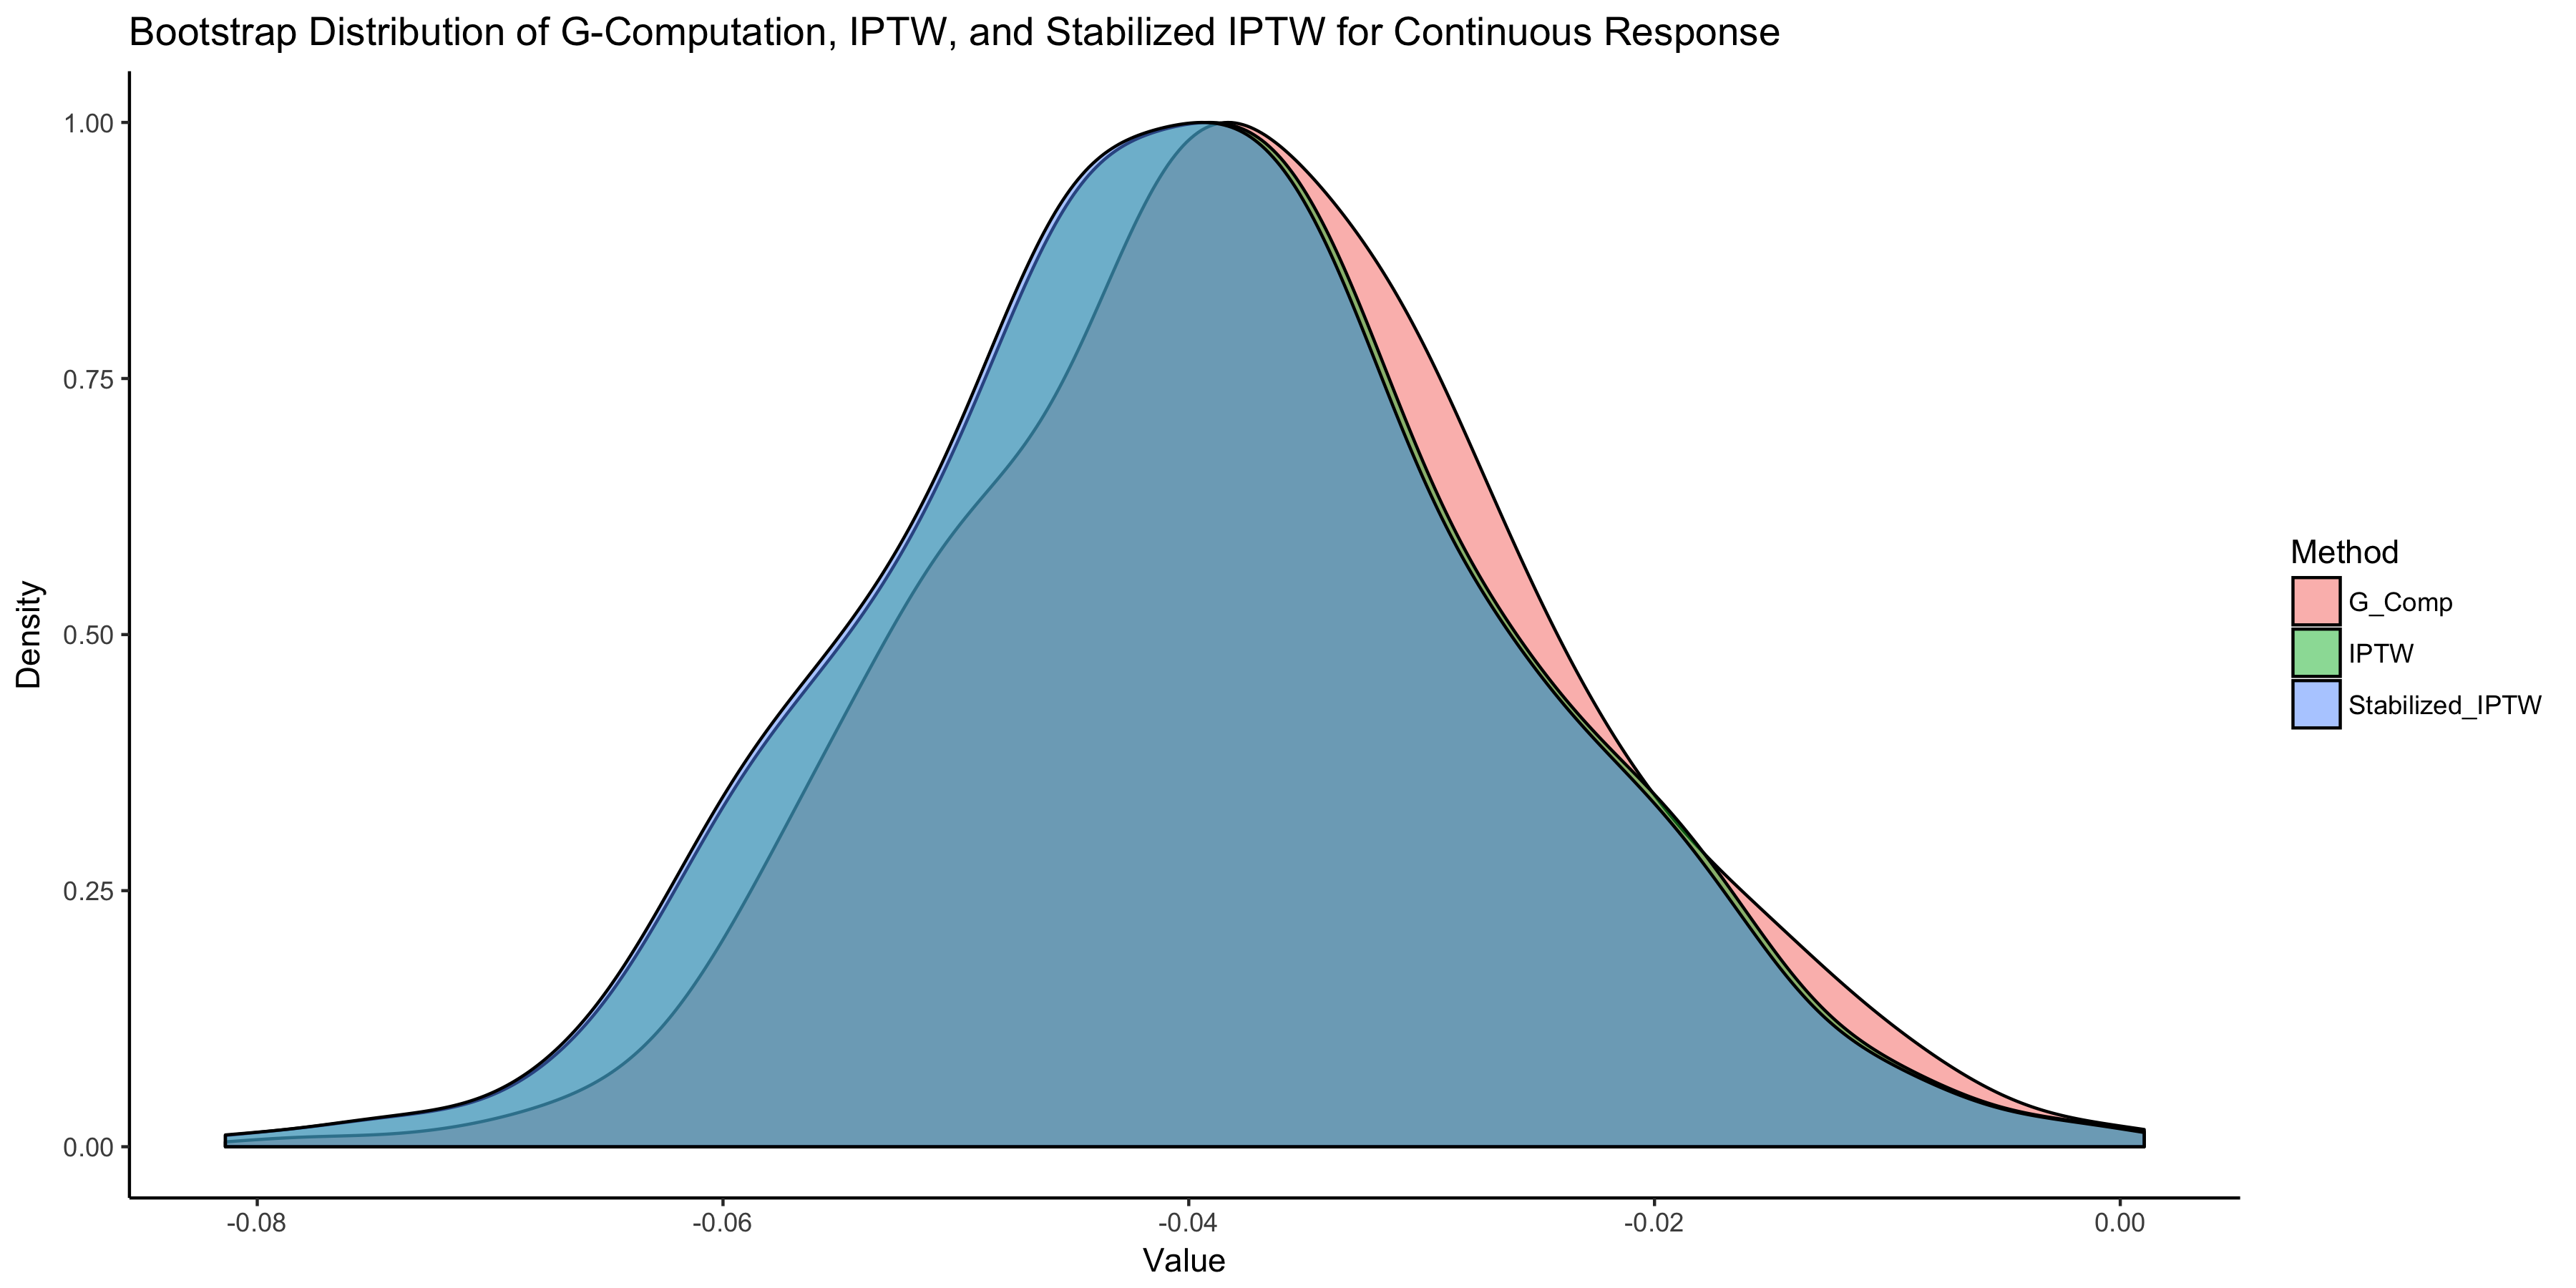
\includegraphics[scale=0.125]{figures/boot_dens_continuous.png}
    \caption{Continuous Response}
    \label{fig:boot_cont}
\end{subfigure}
\caption{Bootstrap Distribution of the Estimates under Binarized and Continuous Response}
\label{fig:boot_dist}
\end{figure}

In Figures \ref{fig:boot_bin} and \ref{fig:boot_cont} we take a look at the bootstrapped distributions for the G-Computation, IPTW, and Stabilized IPTW estimators for both binary and continuous response. They all look relatively similar to each other and are practically normally distributed. This further provides evidence to our suggestion that the large sample size is allowing for well behaved CLT type behavior.

\subsection{Inference}
\begin{table}
\begin{center}
\begin{tabular}{lcc}
\toprule
 & \multicolumn{2}{c}{Outcome} \\ \cmidrule(lr){2-3}
 & \multicolumn{1}{c}{Binary} & \multicolumn{1}{c}{Continuous} \\ \cmidrule(lr){2-2}\cmidrule(lr){3-3}
Estimand  & $p$-value & $p$-value \\ 
\midrule
G-Computation  & $0.0271$ & $\phantom{-}0.00285$ \\
IPTW  & $0.0174$ & $\phantom{-}0.00244$ \\
Stabilized IPTW  & $0.00885$ & $\phantom{-}0.00226$ \\
TMLE & $0.052$ & $\phantom{-}0.0123$ \\
\bottomrule 
\end{tabular}
\caption{$p$-values from Bootstrapped and IC-based Inference}
\label{tab:inference}
\end{center}
\end{table}
In Table \ref{tab:inference}, we see that for all of our hypothesis test except for binary response TMLE, we would reject the null of no average treatment effect. In general, influence curve based inference for TMLE tended to be more conservative in the amount of evidence supplied by the $p$-value to reject the null than the non-parametric based inference. 

\subsection{Discussion}
Based on Tables \ref{tab:estimation} and \ref{tab:inference}, we make the conclusion that under our independence and convenience assumptions, the average treatment effect of hospitalization under the treatment of vaccination is significantly nonzero and in fact negative. For binarized response, we find that there is around a $1\%$ decrease in hospitalization under treatment of vaccination, whereas for the continuous response we find a reduction of about $3-4$ hospitalizations per 100.

We note, however, that influence curve based inference for TMLE tended to be more conservative than bootstrap based estimation for G-Computation, IPTW, and Stabilized IPTW. We ultimately made our conclusion of the significance of the average treatment effect based on the non-parametric bootstrap for a couple reasons. Firstly, because the weights were relatively well behaved and the bootstrapped IPTW and Stabilized-IPTW distributions were so similar, we have reason to believe that along with our large sample size, the non-parametric bootstrap was more accurately able to estimate the sampling distribution of the ATE. Secondly, because of our large sample size, we had to be relatively careful with our SuperLearner library due to computational constraints. We conjecture that had we used a more robust SuperLearner library, the influence curve based inference for TMLE would have been similar to that of the bootstrapped based inference for the other estimators.

\section{Conclusion}
In this analysis, we sought to study the impact of vaccination on subsequent hospitalization among older adults with diabetes. Motivated by existing studies, we sought to frame the question in a causal manner where the intervention of interest was the existence of vaccination. Due to the nature of the data set, in particular that we had a large sample, we were able to construct a very expressive structural causal model, but we also needed to make a few independence and convenience assumptions due to the lack of identifiability.

After doing so, we estimated our causal parameter of interest: the average treatment effect via the G-Computation, IPTW, Stabilized IPTW, and TMLE estimators. When assessing the positivity assumptions, we found that everything was relatively well behaved. We can do so by examining the distribution of propensity scores of the IPTW and stablized IPTW weights. As shown before, we have no particularly extreme weight and the distributions of both the IPTW and stabilized IPTW weights were remarkably similar. We further saw this stability in the actual analysis where the results rather similar and the bootstrap distributions of the estimates were very similar too.

At the end of our analysis, we perform inference and deduce that with strong evidence, vaccination does seem to significantly affect hospitalization among older adults with diabetes. Toward this end, we suggest that older adults get their vaccinations, especially influenza vaccines. There are, however, a few limitations to our study. First, it is the number of convenience assumptions we had to make. Second, the target population is rather limited. This particular population was chosen with the hope of minimizing confounding when possible, so we cannot comment on the validity of the results had this study been replicated on a different target population. 

\subsection{Reproducibility}
In order to reproduce our results, please see the instructions at \url{https://github.com/erickim/PH252D_final_project}.

\subsection{Contributions}
Denys - Brainstorm the project direction; a third of the presentation slides; Sections 1 and 2 in the write up. \\
James - Brainstorm the project direction; half of the coding; a third of the presentation slides; Sections 5, 6.1 in the write up. \\
Eric - Half of the coding; a third of the presentation slides; Sections 3, 4, 6.2-6.4 and 7 in the write up. \\
David - Brainstorm the project direction; acquired the data set.

\begin{thebibliography}{20}

\bibitem{Baxter} Baxter R, Lee J, Fireman B. Evidence of Bias in Studies of Influenza Vaccine Effectiveness in Elderly Patients. {\em J Infect Dis}. 2010; 201(2):186-189. doi:10.1086/649568

\bibitem{Budnitz} Budnitz DS, Lovegrove MC, Shehab N, Richards CL. Emergency Hospitalizations for Adverse Drug Events in Older Americans. {\em N Engl J Med}. 2011; 365(21):2002-2012. doi:10.1056/NEJMsa1103053

\bibitem{CDC1} Centers for Disease Control and Prevention. Recommended Vaccines for Adults. https://www.cdc.gov/vaccines/adults/rec-vac/index.html. Published January 25, 2018. Accessed April 17, 2018.

\bibitem{CDC2} Centers for Disease Control and Prevention. Table 3, Flu Vaccination Coverage by Age Group, Adults 18 Years and Older, United States, 2015-16 Season. https://www.cdc.gov/flu/fluvaxview/coverage-1516estimates.htm. Published November 1, 2017. Accessed April 19, 2018.

\bibitem{Ho} Ho PM, Rumsfeld JS, Masoudi FA, et al. Effect of Medication Nonadherence on Hospitalization and Mortality Among Patients With Diabetes Mellitus. {\em Arch Intern Med}. 2006; 166(17):1836–1841. doi:10.1001/archinte.166.17.1836

\bibitem{Howard} Howard DH, Sentell T, Gazmararian JA. Impact of health literacy on socioeconomic and racial differences in health in an elderly population. {\em J Gen Intern Med}. 2006; 21(8):857-861. doi:10.1111/j.1525-1497.2006.00530.x

\bibitem{Jimenez-Garcia} Jiménez-García R, Jimenez I, Garrido PC, et al. Coverage and predictors of influenza vaccination among adults with diabetes in Spain. {\em Diabetes Res Clin Pract}. 2008; 79(3):510-517. doi:10.1016/j.diabres.2007.10.013

\bibitem{Looijmans} Looijmans-Van den Akker I, Verheij TJM, Buskens E, Nichol KL, Rutten GEHM, Hak E. Clinical Effectiveness of First and Repeat Influenza Vaccination in Adult and Elderly Diabetic Patients. {\em Diabetes Care}. 2006; 29(8):1771-1776. doi:10.2337/dc05-2517

\bibitem{Nichol} Nichol KL, Nordin J, Mullooly J, Lask R, Fillbrandt K, Iwane M. Influenza Vaccination and Reduction in Hospitalizations for Cardiac Disease and Stroke among the Elderly. {\em N Engl J Med}. 2003; 348(14):1322-1332. doi:10.1056/NEJMoa025028

\bibitem{Sun} Sun R, Karaca Z, Wong HS. Trends in Hospital Inpatient Stays by Age and Payer, 2000-2015. Rockville, MD: {\em Agency for Healthcare Research and Quality}; 2018. https://www.hcup-us.ahrq.gov/reports/statbriefs/sb235-Inpatient-Stays-Age-Payer-Trends.jsp. Accessed April 23, 2018.

\bibitem{Vamos} Vamos EP, Pape UJ, Curcin V, et al. Effectiveness of the influenza vaccine in preventing admission to hospital and death in people with type 2 diabetes. {\em Can Med Assoc J}. 2016; 188(14):E342-E351. doi:10.1503/cmaj.151059

\bibitem{Williams} Williams WW, Lu, P., O’Halloran, A., et al. Surveillance of Vaccination Coverage Among Adult Populations — United States, 2015. {\em MMWR Surveill Summ}. 2017; 66(SS-11):1-28. doi:10.15585/mmwr.ss6611a1

\end{thebibliography}
\end{document}